\documentclass[a4paper,12pt]{report}
\usepackage[utf8]{inputenc}
\usepackage{amsmath}
\usepackage{graphicx}
\usepackage{listings}
\usepackage{tikz}
\usepackage[T1]{fontenc}
\usepackage{color}
\usetikzlibrary{arrows,automata}
\definecolor{pythonred}{rgb}{0.6,0,0} % for strings
\definecolor{pythongreen}{rgb}{0.25,0.5,0.35} % comments
\definecolor{pythonpurple}{rgb}{0.5,0,0.35} % keywords
	\definecolor{pythondocblue}{rgb}{0.25,0.35,0.75} % javadoc
	 
	\lstset{language=python,
	basicstyle=\ttfamily,
	keywordstyle=\color{pythonpurple}\bfseries,
	stringstyle=\color{pythonred},
	commentstyle=\color{pythongreen},
	morecomment=[s][\color{pythondocblue}]{/**}{*/},
	numbers=left,
	numberstyle=\tiny\color{black},
        stepnumber=2,
	numbersep=10pt,
	tabsize=4,
	showspaces=false,
	showstringspaces=false}

% Title Page

 \title{\bfseries\huge \textcolor{purple}{\underline {EEP702-Software Lab}} \\{\textcolor{blue}{Assignment 9 : Caculating LCM and GCD using MACROS And Use of gprof}}}
\author{\bfseries\large\textcolor{black}  {Harshit Kumar Gupta}\\ {\textcolor{black} {2013EET2369 }}\\

\includegraphics[width=3cm,height=3.4cm]{./iit.png}\\\noindent Computer Technology\\
\noindent Department Of Electrical Engineering\\IIT DELHI}
% iit.png: 282x282 pixel, 72dpi, 9.95x9.95 cm, bb=0 0 282 282
\begin{document}
\maketitle
\tableofcontents


\chapter{\textcolor{blue}{\underline {PROBLEM STATEMENT}}}
\noindent Optimizing code for speed using inline assembling

PROBLEM 1:

\noindent Given two integers, write a time efficient c code, that spends as less time in memory access
and more in calculations as possible, to get their GCD and LCM.Use directives for conditional
compilation of code as follows. Find the critical parts of code that consume more percentage of time using gprof and replace
those parts with inline assembly coding to optimize speed and compare the time profiling for
both codes. \\\\

PROBLEM 2:
\begin{enumerate}
 \item Find the most significant non zero bit position for largest of the two given integers using pure c code and inline assembled c code and show which one is faster.
 \item Convert the given integer(assumed to be angle in degrees) to radians and find the floating point cosine value with pure c and inline assembled c and determine fastest one using gprof.
 \item Use gprof on the code of assignment no-04 Library management and rewrite the code to optimize time.

\end{enumerate}




\begin{center}
\chapter{\textcolor{blue}{\underline {ABSTRACT}}}
\end{center}
\noindent Basically our Purpose of Implementation is to see where does a Code hangs up or uses
much of memory Space while Execution. The Use of Gprof allows us to ou to learn where your program spent its time and which functions called which other functions while it was executing. This information can show you which pieces of your program are slower than you expected, and might be candidates for rewriting to make your program execute faster. It can also tell you which functions are being called more or less often than you expected.
This may help you spot bugs that had otherwise been unnoticed.
\begin{center}
\chapter{\textcolor{blue}{\underline {INTRODUCTION}}}
\end{center}
\noindent 

Once the program is compiled for profiling, you must run it in order to generate the information that gprof needs.
Simply run the program as usual, using the normal arguments, file names, etc. The program should run normally, producing the same output as usual. 
It will, however, run somewhat slower than normal because of the time spent collecting and the writing the profile data.
The way you run the program--the arguments and input that you give it--may have a dramatic effect on what the profile information shows.
The profile data will describe the parts of the program that were activated for the particular input you use.
For example, if the first command you give to your program is to quit, the profile data will show the time used in initialization and in cleanup, but not much else.
Your program will write the profile data into a file called gmon.out' just before exiting. If there is already a file called gmon.out, its contents are overwritten.
There is currently no way to tell the program to write the profile data under a different name, but you can rename the file afterward if you are concerned that 
it may be overwritten.
In order to write the gmon.out' file properly, your program must exit normally: by returning from main or by calling exit. Calling the low-level function 
exit does not write the profile data, and neither does abnormal termination due to an unhandled signal.
The gmon.out file is written in the program's current working directory at the time it exits. This means that if your program calls chdir,
the `gmon.out' file will be left in the last directory your program chdir'd to. If you don't have permission to write in this directory,
the file is not written, and you will get an error message.

\begin{center}
\chapter{\textcolor{blue}{\underline {SPECIFICATIONS AND ASSUMPTIONS}}}
\end{center}
\section*{Specifications}

\begin{enumerate}
\item Entire Code has been made in C Language.
\item Macros have been Explicitly Designed for LCM and HCF.
\item "lcm" function has been used to Compute LCM calling up the "gcd" Function.
\item gprof has been used for code analysis and Optimisation.

\end{enumerate}

\section*{Assumptions}

\begin{enumerate}
\item The Mathematical functions used are Bug-Free.
\item gmon.out is generated on the same path as of the C code.
\item User succesfully enters a Positive values for LCM and HCF Calculation.

\end{enumerate}
 
\begin{center}
\chapter{\textcolor{blue}{\underline {LOGIC USED/METHODOLOGY}}}
\end{center}
The methodology that is used for developing the program is defined below:\\

\begin{enumerate}
\item We intially Design a Proper C code for Calculating both the Values.
\item Below the Header Files Macros are Provided for LCM and HCF.
\item In the (define) Tag we put a Suitable Macro which determines what has to run.
\item The Program may Output the values Very fast as the Code is not quite Complex.
\item We run the gprof Command to our C Code which generates a File named gmon.out
\item It contains  the run time of our and may be Varied increasing the Complexity of our code.
\item Results are Suitably saved in a File.
\end{enumerate}



\begin{center}
\chapter{\textcolor{blue}{\underline {FLOWCHART}}}
\end{center}
\noindent \\Flowchart
\begin{center}
 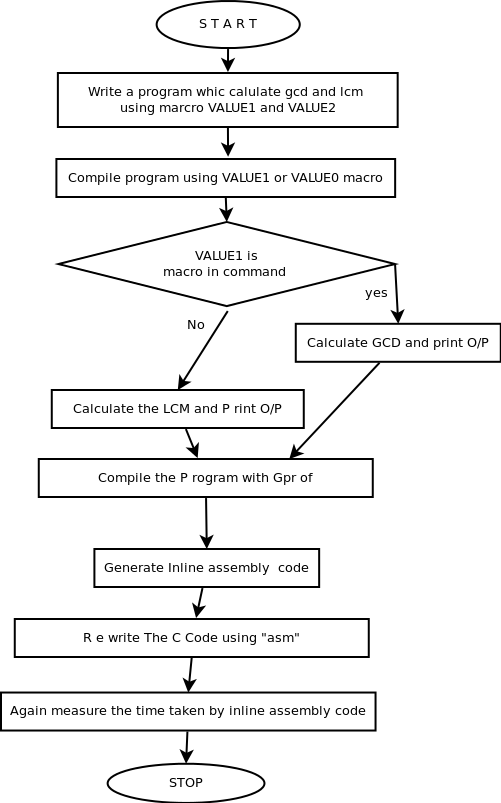
\includegraphics[width=13 cm,height=12 cm]{./flowchart.png}
 % flowchart.png: 239x684 pixel, 72dpi, 8.43x24.13 cm, bb=0 0 239 684
\end{center}


\begin{center}
\chapter{\textcolor{blue}{\underline {EXECUTION DIRECTIVE}}}
\end{center}

 For program following instructions are used.
 \begin{enumerate}
  \item gcc -MACRO pureCcode.c -o test
  \item test
  \item gprof options [executable-file [profile-data-files...]] [> outfile]
\item gprof test gmon.out 
   \item gcc -MACRO InlneAssemblyCode.c -o test
  \item test
 
\item gprof test gmon.out  
 \end{enumerate}



\begin{center}
\chapter{\textcolor{blue}{\underline {RESULTS AND CONCLUSIONS}}}\end{center}
 \begin{enumerate}
  \item  For the Given Conditions Program runs Successfully and Generates a bug free Output.
\item The Profiling is Done with the Help of gprof which returns Satisfactory Outputs.
\item Writing inline assembly code does not always reduce the time taken beacuse sometimes  compiler generate more optimized code 
which we can not  write using assembly.  

 \end{enumerate}
 For the Given Conditions Program runs Successfully and Generates a bug free Output.
The Profiling is Done with the Help of gprof which returns Satisfactory Outputs.\\

\end{center}
\begin{center}
\chapter{\textcolor{blue}{\underline {PROFILING Results}}}
\end{center}

\begin{center}
 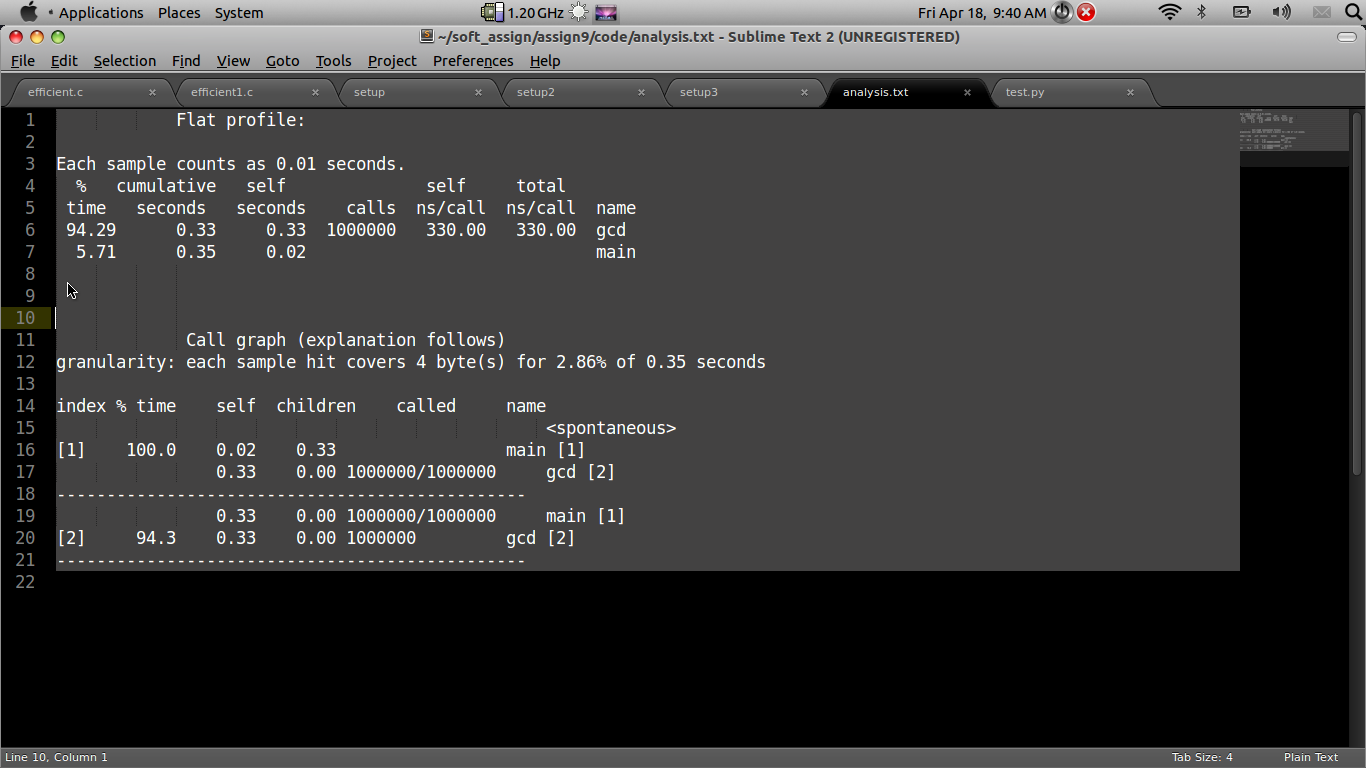
\includegraphics[width=13 cm,height=12 cm]{./gcd.png}
 % flowchart.png: 239x684 pixel, 72dpi, 8.43x24.13 cm, bb=0 0 239 684
profiling  for GCD in c  
\end{center}
\begin{center}
 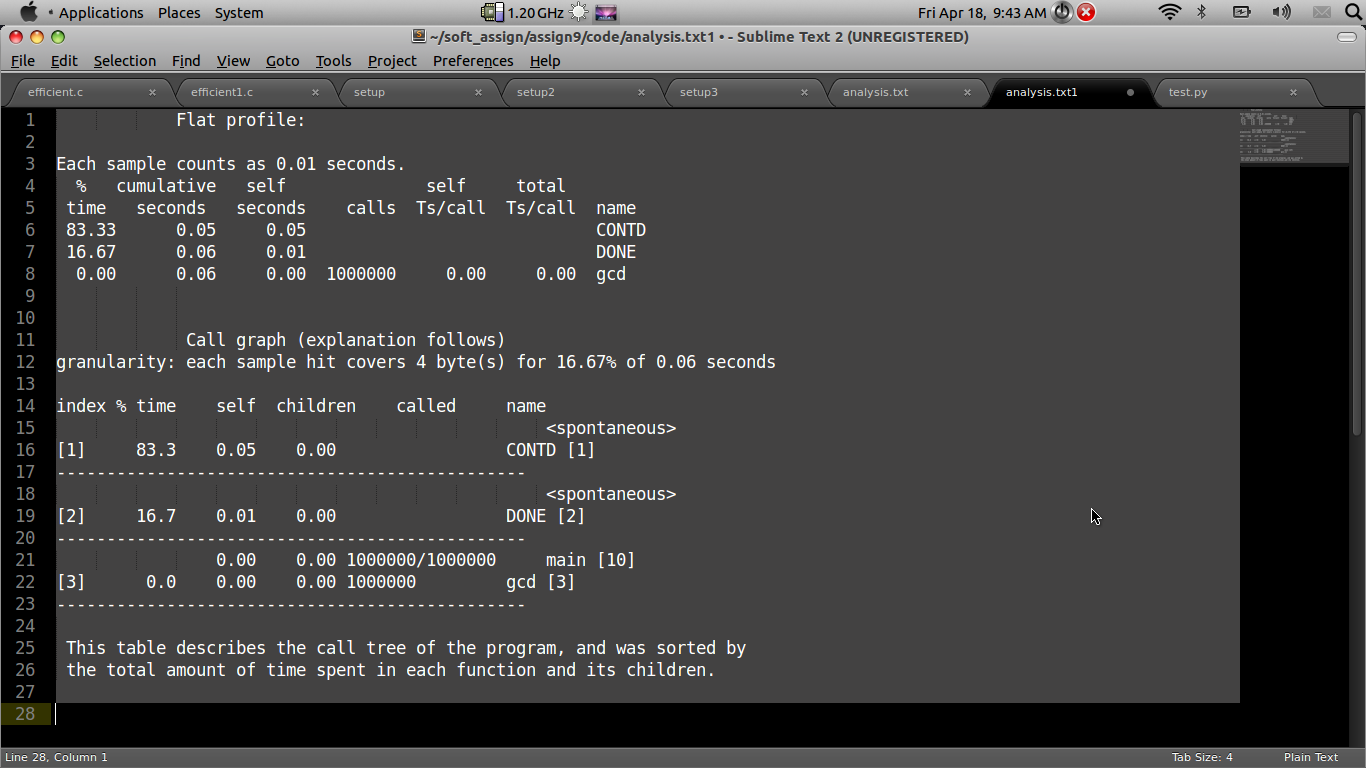
\includegraphics[width=13 cm,height=12 cm]{./gcd1.png}
 % flowchart.png: 239x684 pixel, 72dpi, 8.43x24.13 cm, bb=0 0 239 684
profiling  for GCD in inline assembly
\end{center}
\begin{center}
 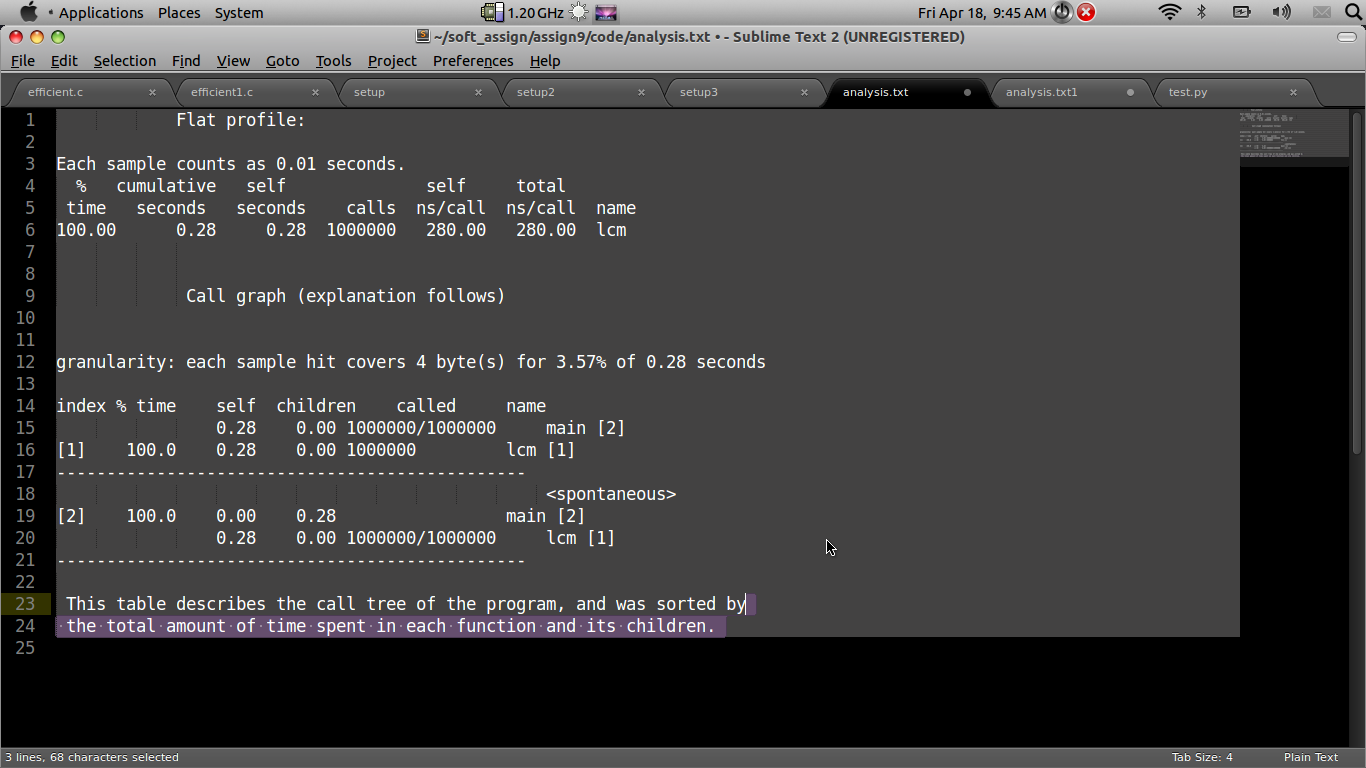
\includegraphics[width=13 cm,height=12 cm]{./lcm.png}
 % flowchart.png: 239x684 pixel, 72dpi, 8.43x24.13 cm, bb=0 0 239 684
profiling  for LCM in C
\end{center}
\begin{center}
 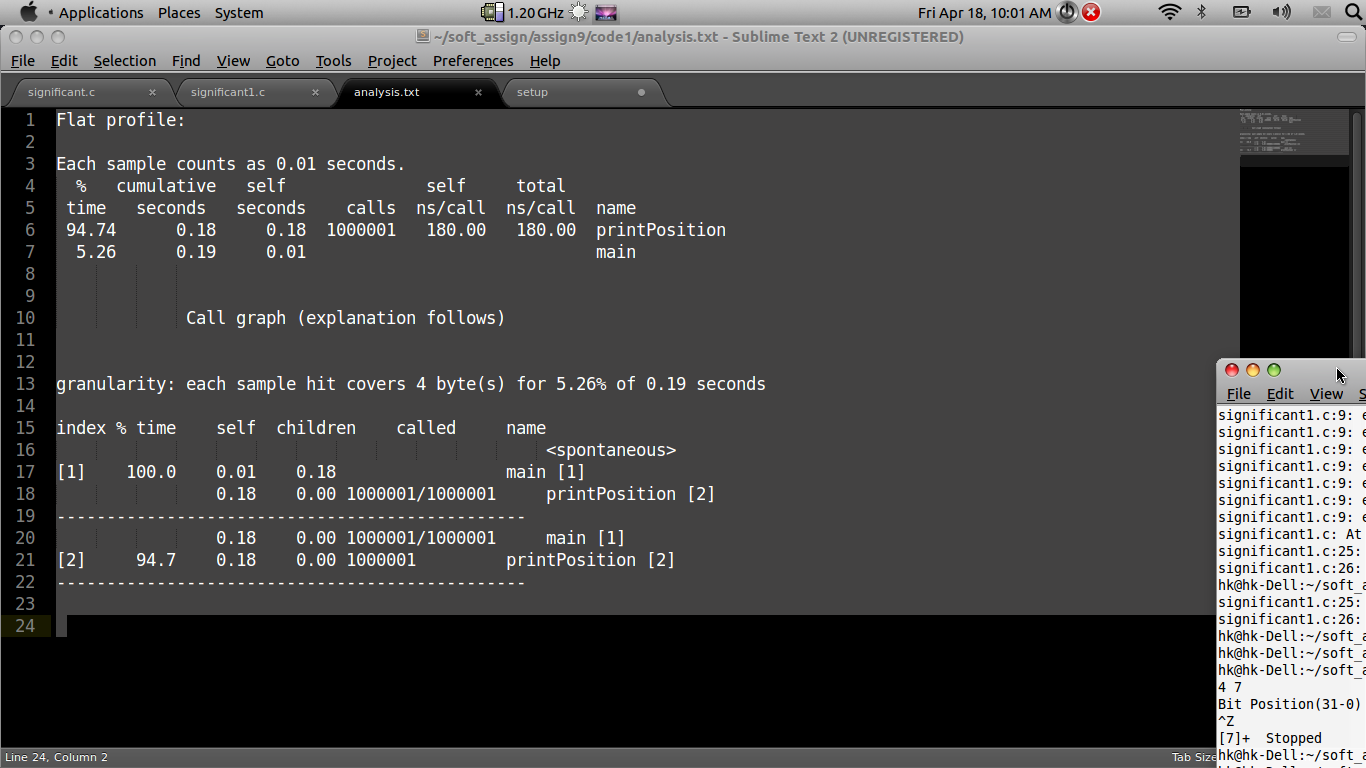
\includegraphics[width=13 cm,height=12 cm]{./significant.png}
 % flowchart.png: 239x684 pixel, 72dpi, 8.43x24.13 cm, bb=0 0 239 684
profiling  for significant bit  in C
\end{center}
\begin{center}
 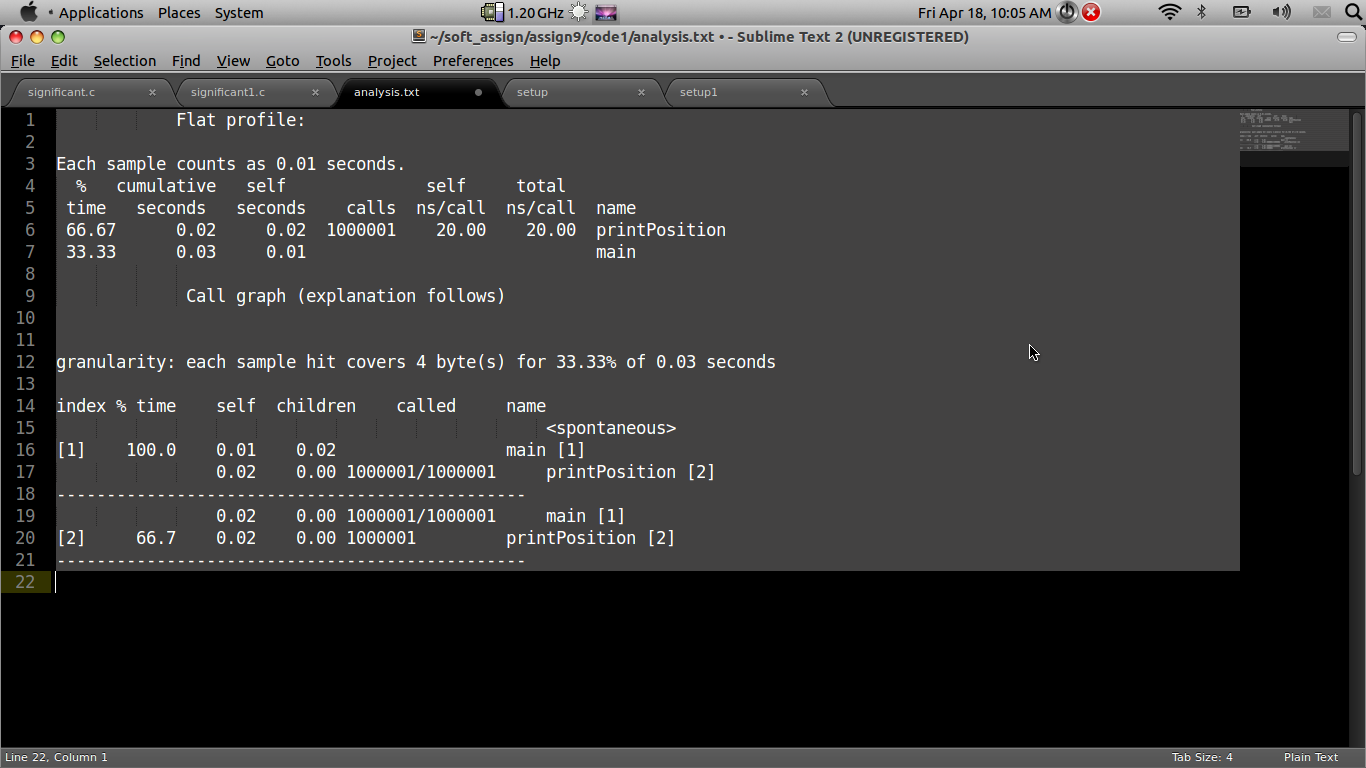
\includegraphics[width=13 cm,height=12 cm]{./significant1.png}
 % flowchart.png: 239x684 pixel, 72dpi, 8.43x24.13 cm, bb=0 0 239 684
profiling  for significant bit in inline assembly.
\end{center}
\begin{center}
 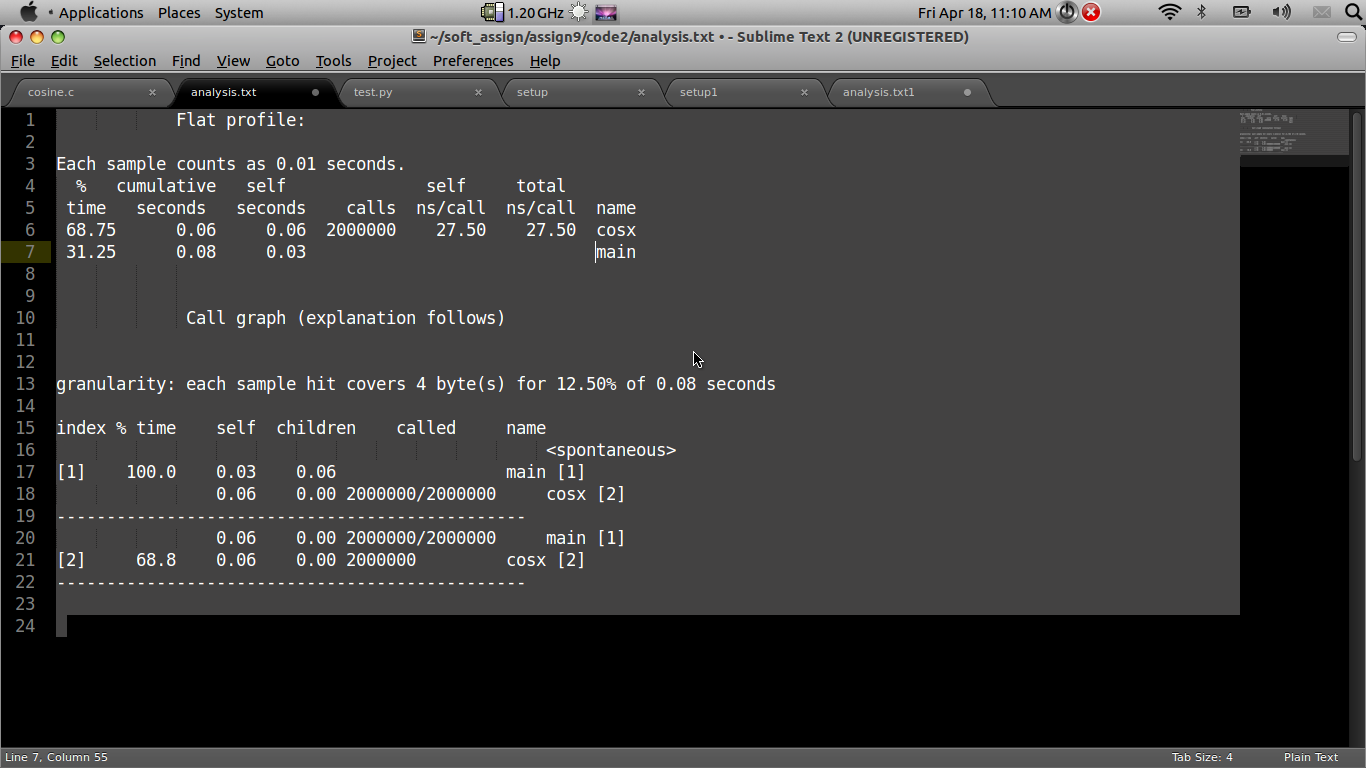
\includegraphics[width=13 cm,height=12 cm]{./cosine.png}
 % flowchart.png: 239x684 pixel, 72dpi, 8.43x24.13 cm, bb=0 0 239 684
profiling for cosine in c
\end{center}
\begin{center}
 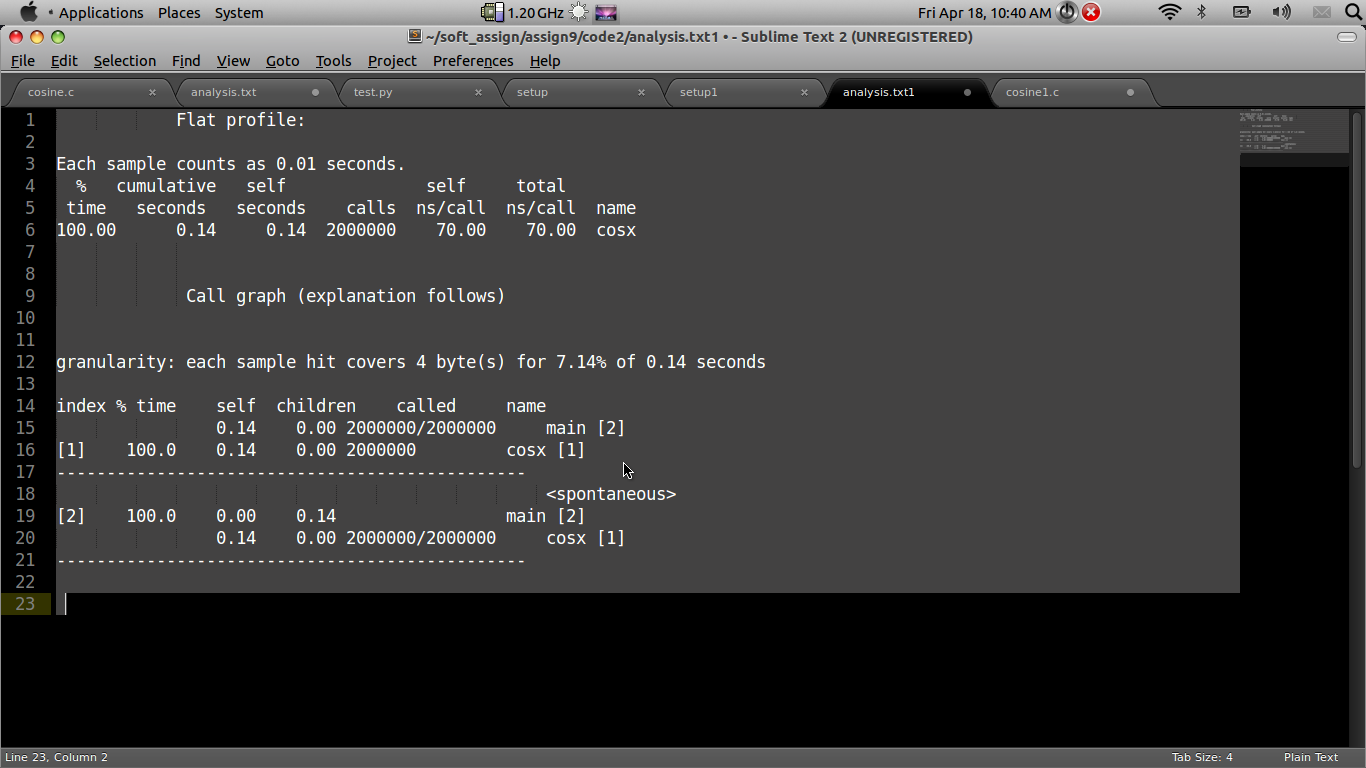
\includegraphics[width=13 cm,height=12 cm]{./cosine1.png}
 % flowchart.png: 239x684 pixel, 72dpi, 8.43x24.13 cm, bb=0 0 239 684
profiling for cosine in inline assembly
\end{center}
\begin{center}
 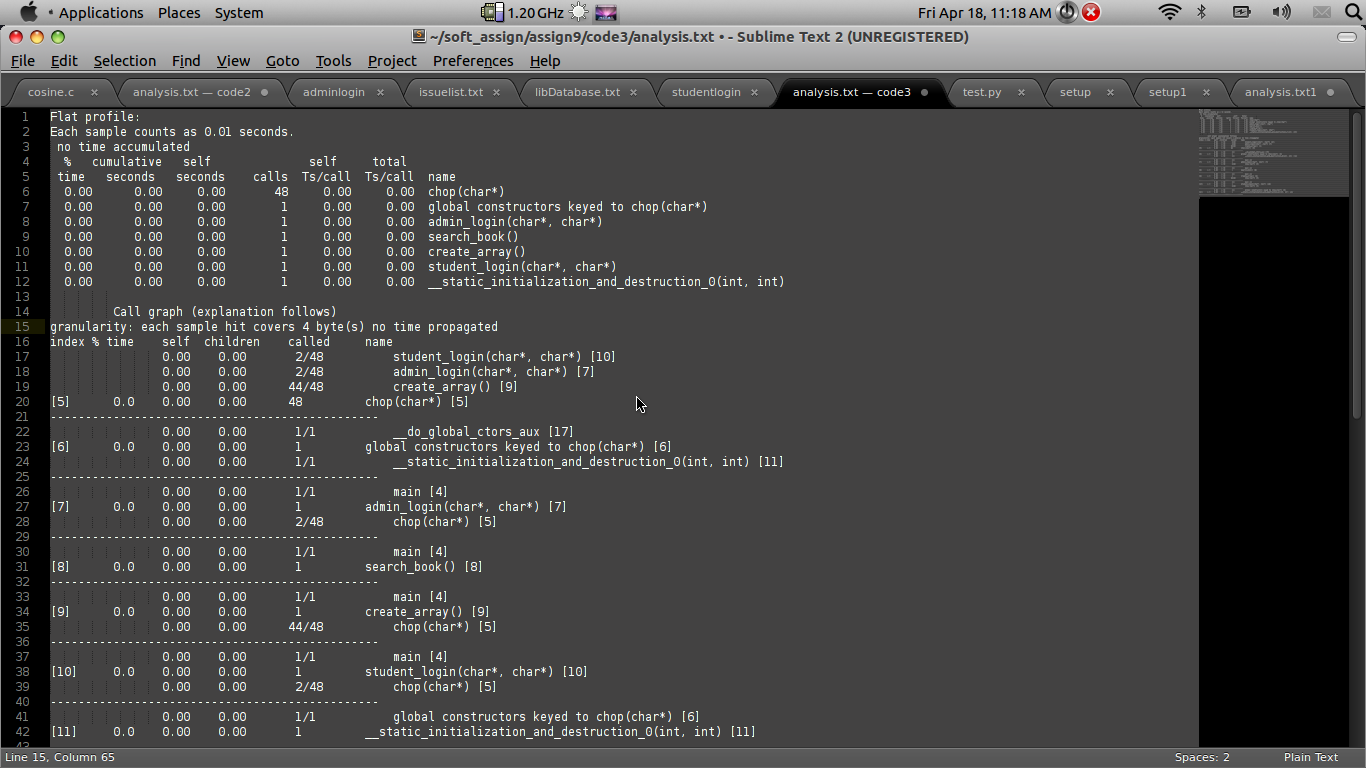
\includegraphics[width=13 cm,height=12 cm]{./library.png}
 % flowchart.png: 239x684 pixel, 72dpi, 8.43x24.13 cm, bb=0 0 239 684
profiling for library management assignment
\end{center}
\end{document}  